\begin{figure*}[!htbp]
\begin{minipage}[c]{0.33\textwidth}
  \vspace{0.1em}
  \centering
  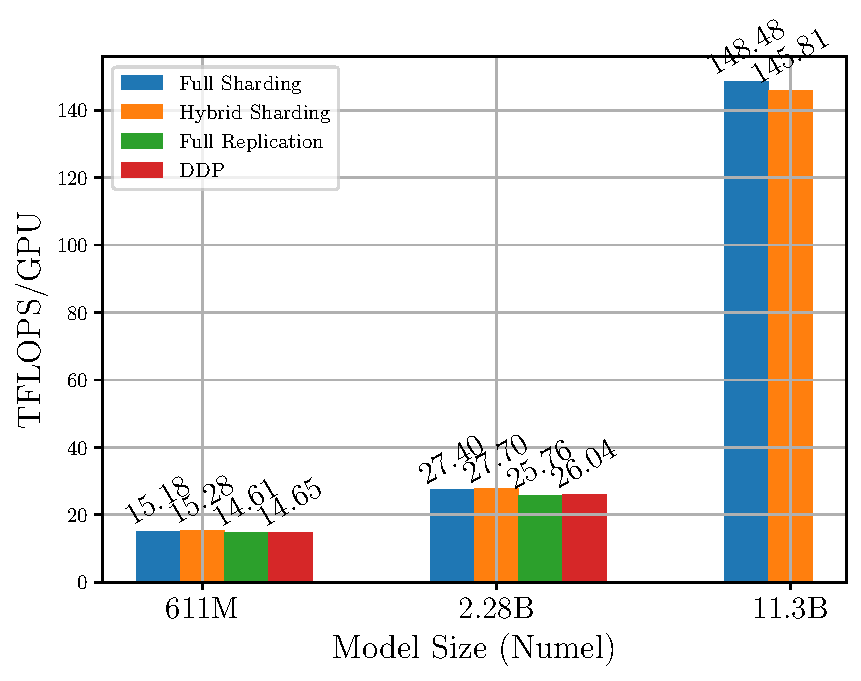
\includegraphics[width=\linewidth]{figure/sharding_strategies.pdf}
  (a) Model Scale
\end{minipage}
\begin{minipage}[c]{0.33\textwidth}
  \vspace{1em}
  \centering
  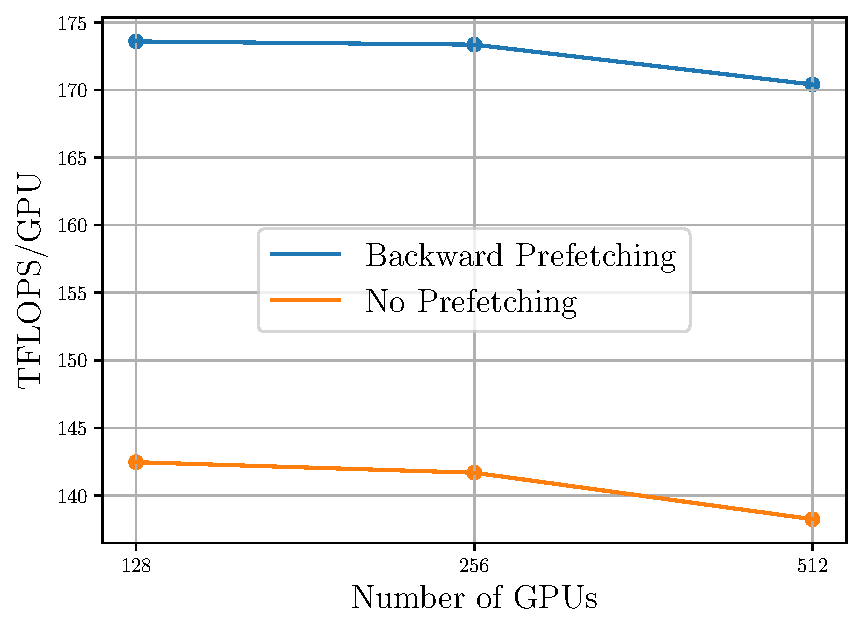
\includegraphics[width=\linewidth]{figure/prefetching_tflops.pdf}
  (b) GPT-175B Backward Prefetch
\end{minipage}
\begin{minipage}[c]{0.33\textwidth}
  \centering
  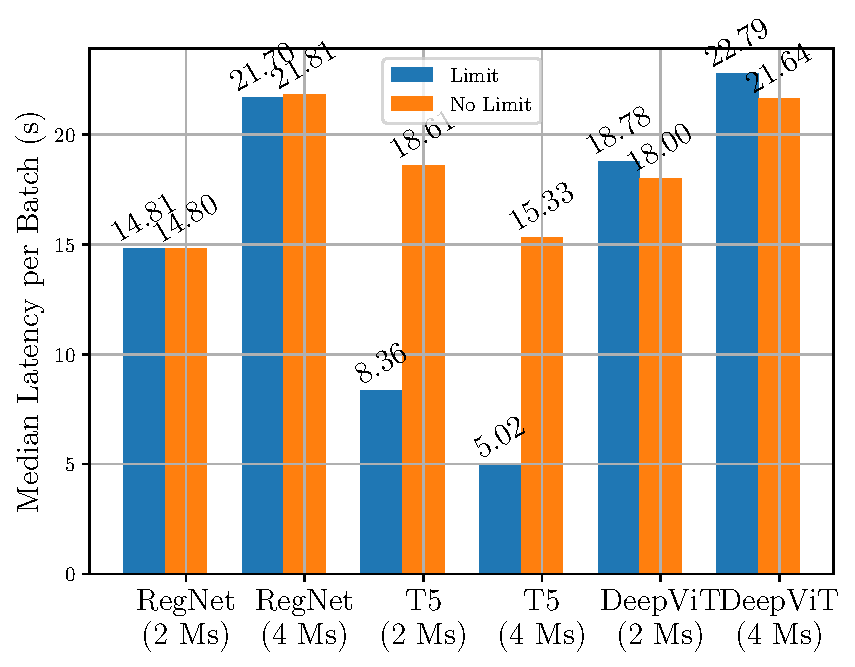
\includegraphics[width=\linewidth]{figure/rate_limiter_latency.pdf}
  (c) Rate Limiter (Ms = Machines)
\end{minipage}
%\vspace{-1em}
\caption{Model Scale and Training Efficiency}\label{fig:mix}
%\vspace{-1em}
\end{figure*}

\subsection{Experiment Setup}\label{sec:exp_setup}

In these experiments, we conducted evaluations on the HuggingFace T5-11B transformer~\cite{raffel2020exploring}, minGPT-175B transformer~\cite{gpt3}, and DHEN recommendation model~\cite{DHEN}. The recommendation models consist of 768B sparse parameters and 550M dense parameters, the sparse parameter tensors were sharded using the first approach mentioned in Section 2.3, which communicates activations instead of parameters, while the dense parameters were trained using FSDP on 8 to 512 A100 80GB GPUs interconnected by a 2Tb/s RoCE network. The objective was to assess the capability and scalability of FSDP in training large-scale models. Additionally, we employed T5-611M, T5-2B and T5-11B transformers to evaluate the performance of various sharding strategies, communication efficiency of prefetching, and communication throttling using rate limiter. Metrics employed in these experiments included TFLOPS per GPU, latency per batch, peak memory allocated, peak memory active, and peak memory reserved.